\documentclass[msc,lith,englisho]{liuthesis}


%%% settings.tex --- 
%% 
%% Filename: settings.tex
%% Description: 
%% Author: Ola Leifler
%% Maintainer: 
%% Created: Tue Oct 19 21:11:31 2010 (CEST)
%% Version: $Id$
%% Version: 
%% Last-Updated: Tue Apr 25 08:49:48 2017 (+0200)
%%           By: Ola Leifler
%%     Update #: 43
%% URL: 
%% Keywords: 
%% Compatibility: 
%% 
%%%%%%%%%%%%%%%%%%%%%%%%%%%%%%%%%%%%%%%%%%%%%%%%%%%%%%%%%%%%%%%%%%%%%%
%% 
%%% Commentary: 
%% 
%% 
%% 
%%%%%%%%%%%%%%%%%%%%%%%%%%%%%%%%%%%%%%%%%%%%%%%%%%%%%%%%%%%%%%%%%%%%%%
%% 
%%% Change log:
%% 
%% 
%% RCS $Log$
%%%%%%%%%%%%%%%%%%%%%%%%%%%%%%%%%%%%%%%%%%%%%%%%%%%%%%%%%%%%%%%%%%%%%%
%% 
%%% Code:

\usepackage[backend=biber,hyperref]{biblatex}
%% To set the font of your thesis, use the \setmainfont{} command,
%% surrounded with \ifxetex if you want to switch between xelatex and pdflatex
\ifxetex 
%\setmainfont [Scale=1]{Georgia}
\fi

%%%%%%%%%%%%
%% The VZ43 chapter style, from Memoir contributed chapter styles: ftp://ftp.tex.ac.uk/ctan%3A/info/MemoirChapStyles/MemoirChapStyles.pdf
%%%%%%%%%%%

\usepackage{calc,color}
\newif\ifNoChapNumber
\newcommand\Vlines{%
\def\VL{\rule[-2cm]{1pt}{5cm}\hspace{1mm}\relax}
\VL\VL\VL\VL\VL\VL\VL}
\makeatletter
\setlength\midchapskip{0pt}
\makechapterstyle{VZ43}{
\renewcommand\chapternamenum{}
\renewcommand\printchaptername{}
\renewcommand\printchapternum{}

\renewcommand\chapnumfont{\Huge\bfseries\centering}
\renewcommand\chaptitlefont{\Huge\bfseries\raggedright}
\renewcommand\printchaptertitle[1]{%
\Vlines\hspace*{-2em}%
\begin{tabular}{@{}p{1cm} p{\textwidth-3cm}}%
\ifNoChapNumber\relax\else%
\colorbox{black}{\color{white}%
\makebox[.8cm]{\chapnumfont\strut \thechapter}}
\fi
& \chaptitlefont ##1
\end{tabular}
\NoChapNumberfalse
}
\renewcommand\printchapternonum{\NoChapNumbertrue}
}
\makeatother


%% To set bibliography options, refer to the biblatex manual and use
%% the ExecuteBibliographyOptions command below to set your options

\ExecuteBibliographyOptions{maxnames=99}


%% Change this to your appropriate BibTeX reference file (.bib)

\addbibresource{references.bib}

%%%%%%%%%%%%%%%%%%%%%%%%%%%%%%%%%%%%%%%%%%%%%%%%%%%%%%%%%%%%%%%%%%%%%%
%%% settings.tex ends here

%%% Local Variables: 
%%% mode: latex
%%% TeX-master: "demothesis"
%%% End: 


% Packages
\usepackage{rotating}
\usepackage{color}
\usepackage{float}


% Notation
\newcommand{\len}{\text{length}}
\newcommand{\dur}{\text{duration}}
\newcommand{\traj}{T}
\newcommand{\obs}{x}
\newcommand{\newobs}{\bar{x}}
\newcommand{\synchedobs}{X}
\newcommand{\timespace}{t}
\newcommand{\synchspace}{\tau}
\newcommand{\statespace}{S}
\newcommand{\posspace}{S'}
\newcommand{\modelf}{f}
\newcommand{\synchf}{g}
\newcommand{\predf}{h}
\newcommand{\model}{\mathcal{M}}
\newcommand{\arrtime}{t}

\department{Institutionen för datavetenskap}
\departmentenglish{Department of Computer and Information Science}
\departmentshort{IDA}
\supervisor{Mattias Tiger}
\examiner{Fredrik Heintz}
\titleenglish{Trajectory-based Arrival Time Prediction using Gaussian Processes}
\subtitleenglish{}
\titleswedish{Trajektoriebaserad ankomsttidsprediktion med Gaussiska Processer}
\thesissubject{Datateknik}
\publicationyear{2019}
\currentyearthesisnumber{001}
\dateofpublication{2019-05-08}
\author{Sebastian Callh}


\begin{document}
\chapterstyle{VZ43}
% Created 2019-01-08 tis 15:58
% Intended LaTeX compiler: pdflatex
\documentclass[11pt]{article}
\usepackage[utf8]{inputenc}
\usepackage[T1]{fontenc}
\usepackage{graphicx}
\usepackage{grffile}
\usepackage{longtable}
\usepackage{wrapfig}
\usepackage{rotating}
\usepackage[normalem]{ulem}
\usepackage{amsmath}
\usepackage{textcomp}
\usepackage{amssymb}
\usepackage{capt-of}
\usepackage{hyperref}
\author{Sebastian}
\date{\today}
\title{}
\hypersetup{
 pdfauthor={Sebastian},
 pdftitle={},
 pdfkeywords={},
 pdfsubject={},
 pdfcreator={Emacs 26.1 (Org mode 9.1.9)}, 
 pdflang={English}}
\begin{document}

\tableofcontents

\section{Introduction\hfill{}\textsc{intro}}
\label{sec:org2505a3f}
The introduction shall be divided into these sections:

\subsection{Motivation\hfill{}\textsc{motivation}}
\label{sec:org96150aa}
As the years pass, more and more people move into urban areas and this
increases the importance of sustainable urban development. A greater
number of inhabitants puts higher pressure on the public
transportation systems, which makes their efficiency increasingly
important.\textasciitilde{}\cite{kondepudi2014smart} 

To offer a better service, public traffic providers use systems
that predict arrival times of buses, trains and similar vehicles. The
accuracy of these predictions are paramount, since many people depend
on these services and erroneous predictions reflects badly on the
public traffic providers. 

Various machine learning algorithms have been applied with great
promise to predict arrival time  \cite{Kim2011Nov}, \cite{RNNBusPredictions} \textasciitilde{}\cite\{zheng2013urban, kim2017probabilistic, pang2018learning,
Nguyen2018Jun\}, although it is still an active research area.

\subsection{Aim\hfill{}\textsc{aim}}
\label{sec:orge66327a}
\subsection{Research questions\hfill{}\textsc{questions}}
\label{sec:org29bb77d}
\subsection{Delimitations\hfill{}\textsc{delimitations}}
\label{sec:org5d92b72}
\subsection{Report outline\hfill{}\textsc{outline}}
\label{sec:org31ec55d}
\end{document}

\chapter{Background}
This chapter describes theoretic results that this thesis is based
on. It covers trajectory data, supervised machine learning from a
Bayesian perspective, GPs, and arrival time prediction using machine learning.

\section{Trajectory Data}
A \textit{trajectory} $\traj_{k}$ of can be seen as an ordered collection of
observations $(\obs^{(k)}_1, \obs^{(k)}_2, \dots, \obs^{(k)}_N)$.
The thesis project focuses on \textit{spatio-temporal}
trajectories, which mean that each observation in a trajectory has a position both in time
and in space. A trajectory has a \textit{length} and
a \textit{duration}. The length $\len(\traj_{k}) = N$ is the number of
observations, and the duration $\dur(\traj_{k}) = \text{time}(\obs^{(k)}_N) - \text{time}(\obs^{(k)}_1)$
is the time from the first observation to the last.
These properties are in general not the same for different
trajectories, which makes it hard to compare them in a
meaningful way. Having different lengths makes a comparison
particularly difficult. If a set of trajectories all have the same length, they could
be viewed as vectors, with one observation per dimension, and compared
using Euclidian distance. But trajectories of different lengths do not
exist in the same vector space, so Euclidian distance fails and more
advanced similarity metrics have to be used.
An illustration of trajectories with different length can be seen in Figure~\ref{fig:trajectory-projection-problems}.
\begin{figure}
  \centering
  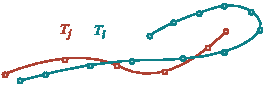
\includegraphics[width=0.7\textwidth]{figures/trajectory-projection-problems}
  \caption{An illustration of two trajectories $\traj_{i}$ and $\traj_{j}$
    with different lengths and duration. There is no natural way of
    measuring the distance between them.}\label{fig:trajectory-projection-problems}
\end{figure}

\section{Supervised Machine Learning}
Supervised machine learning is the process of training computers programs to
recognise patterns in data~\ref{Bishop-2006}. It is incredibly
flexible, and can find patterns such as ``What
temperature is expected for this time of year on this geographical
position?'' or ``What subject is this text about?''. Finding the first
type of pattern of continuous temperature is called
\textit{regression}, and finding the
second pattern with a discrete number of subjects is called
\textit{classification}. Both types of problems have two inputs: 
the \textit{observations}
\[X =
  \begin{pmatrix}
    \obs_{1}^{1} & \obs_{2}^{1} & \cdots & \obs_{D}^{1} \\
    \obs_{1}^{2} & \obs_{2}^{2} & \cdots & \obs_{D}^{2} \\
    \vdots  & \vdots  & \ddots & \vdots  \\
    \obs_{1}^{N} & \obs_{2}^{N} & \cdots & \obs_{D}^{N} \\
  \end{pmatrix},
\]
containing $N$ observations, and the \textit{target vector} $Y = (y_{1},
y_{2}, \dots, y_{N})$. In the first example of predicting temperatures,
$X$ could contain rows of latitude, longitude and time of year, and $Y$ the
corresponding recorded temperatures. The
goal is to learn how the input and output is related by finding a model which approximates a $D$-ary function $y_n =
f(\obs_n)$ for $1 \leq n \leq N$. Such a model could then
predict $y$ for a previously unseen input $\hat{\obs}$. The way a
model approximates $f$ depends entirely on the model, of which there
are many. Common for all models however, is that they are all \textit{trained}
on data. It is during this process they learn the patterns in the data
which they then use to make predictions.
While there are many approaches to this, the remainder of this
section describes the process of selecting and training models,
and using them to make predictions from a Bayesian point of view.

\subsection{Model Training}
The first step is to pick a model for the data, which in a Bayesian
framework is a probability distribution $\prob(\obs \vert \hyperparam)$, where
$\hyperparam$ is a hyper-parameter vector to the distribution. The
probability of all observations is then $\prob(X \vert \hyperparam) =
\prob(\obs_1, \obs_2, \dots, \obs_N \vert \hyperparam)$. For
mathematical convenience it is often assumed that the observed data
come from the same distribution and that each observation is
independent of all other. This means that the probability of a pair of observations $\obs_i$, $\obs_j$ is $\prob(x_i, x_j
\vert \hyperparam) = \prob(\obs_i \vert \hyperparam)\prob(\obs_j
\vert \hyperparam)$ and consequently, that the probability of observing all the data
is $\prob(X \vert \hyperparam) = \prod_{i=1}^N\prob(\obs_i \vert \hyperparam)$.
This is known as the \textit{likelihood}, which describes how likely
the data is given a certain $\hyperparam$. One way of training a model is
by finding $\hat{\hyperparam} = \underset{\hyperparam}{\mathrm{argmax}}$ $\prob(X \vert \hyperparam)$, 
which is called \textit{maximum likelihood}-estimation (ML-estimation), since it picks the
$\hyperparam$ that maximises the likelihood of the data. However, this picks a single
``best value'', highly sensitive to the choice of training data, which
can lead to a problem called \textit{over-fitting}.

\begin{figure}
  \begin{minipage}{.46\textwidth}
    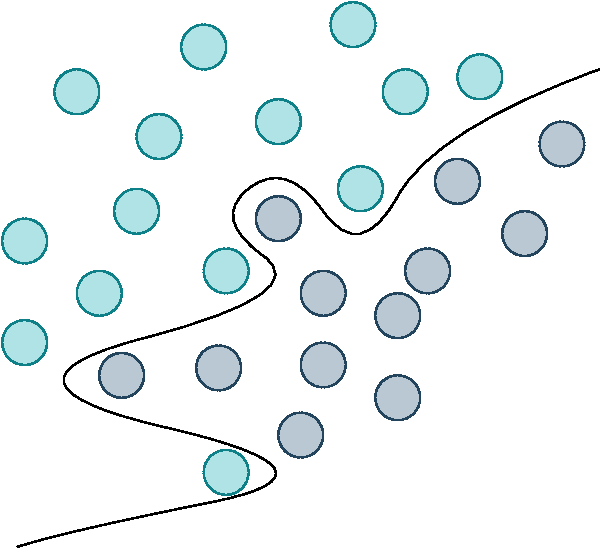
\includegraphics[scale=0.5,width=\textwidth]{figures/over-fit-example}
    \caption{Example of an over-fit in a classification problem. The
      function separating the two classes is too flexible, and captures observations
      which should be consider noise. This model will not generalise well. }\label{fig:over-fit-example}
  \end{minipage}
  \hspace{5pt}
  \begin{minipage}{.46\textwidth}
    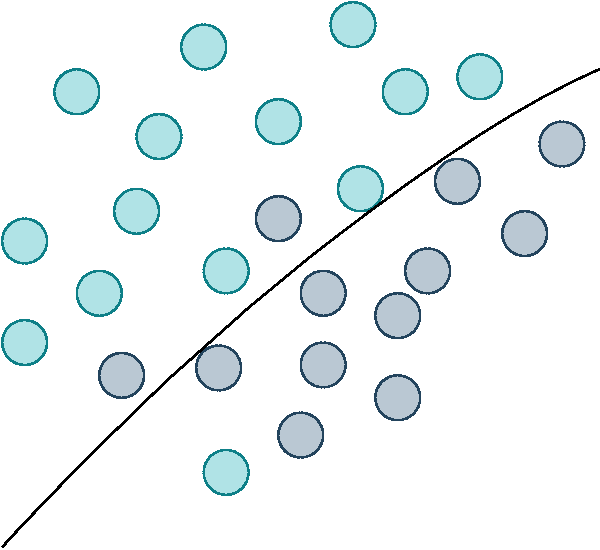
\includegraphics[scale=0.48,width=\textwidth]{figures/good-fit-example}
    \caption{Example of a good fit in a classification problem. The
      function separating the two classes captures the generale structure of the
      data. Even though this misclassifies some observations, this
      model stands a much better chance at generalising.}\label{fig:good-fit-example}
  \end{minipage}
\end{figure}

The goal when training a model is to learn patterns that
\textit{generalise} to unseen data. If $\hyperparam$ is estimated
from data using ML-estimation, it is possible to find a $\hat{\hyperparam}$ that
makes for an increadibly flexible model which \textit{perfectly}
captures the patterns in the data. However, it is very common for data
to contain noise and outliers, which do not represent a pattern that
generalise well. A model that learns these is said to have
\textit{over-fit}, which is highly undesireable. An illustration of
this can be seen in Figure~\ref{fig:over-fit-example}, together with Figure~\ref{fig:good-fit-example}.

One way of avoiding over-fitting is to use \textit{Bayesian inference}, in which 
Bayes theorem
\begin{equation}
  \label{eq:bayes}
  \prob(\hyperparam \vert X) = \frac{\prob(X \vert \hyperparam) \prob(\hyperparam)}{\prob(X)}
\end{equation}
is used to estimate $\hyperparam$ from the \textit{posterior} distribution $\prob(\hyperparam \vert X)$.
This process is called \textit{maximum a posteriori}-estimation (MAP-estimation). To use Bayes
rule a \textit{prior} distribution $\prob(\hyperparam)$ is required, which formalises
a prior belief about $\hyperparam$ before observing any data. The prior is
subjective, and different people may pick different priors,
representing their personal belief about the data. By picking a
prior corresponding to a not-too-flexible model, over-fitting can be
avoided. In the case of GPs, this corresponds to a distribution over kernel
parameter $\hyperparam$ which gives a very wide
kernel. This implies a high correlation between observations further
apart, which in turn implies a slowly-varying function.
In summary, the process of training a model is equivalent to computing
the posterior, from which the most probable model parameters can be
extracted. Training a model using ML- or MAP-estimation both require that the
likelihood can be optimised. This is not always possible to do in
closed form, in which case iterative methods, such as Stochastic
Gradient Descent (SGD) can be used. These types of methods are
prone to to finding local optimas, so random restarts need to be used
to increase the chances of finding a good parametrisation.

If a prior is specified, it is possible to estimate the parameters of
model $\model$ \textit{without} fitting it to data, avoiding the
problem of over-fitting entirely. This is done by maximising the
\textit{marginal likelihood}
\begin{equation}
  \label{eq:marginal-likelihod}
  \prob(\obs \vert \model) = \int \prob(\obs \vert \hyperparam,
  \model) \prob(\hyperparam \vert \model) \prop(\hyperparam) d\hyperparam
\end{equation}
which considers both the uncertainty in $\obs$ and
$\hyperparam$. However, the marginal likelihood is very sensitive to
the choice of prior, so if the prior is not selected carefully this
way of estimating $\hyperparam$ will produce a bad model. The integral
can also be intractable to compute.

\subsection{Making Predictions}
When the model is trained, it can be used to make predictions
about new observations, via the \textit{posterior
  predictive distribution}
\begin{equation}
  \label{eq:posterior-predictive}
  \prob(y \vert X) = \int \prob(y|X,\hyperparam)\prob(\hyperparam \vert X) d \hyperparam,
\end{equation}
\begin{figure}
  \begin{minipage}{.46\textwidth}
    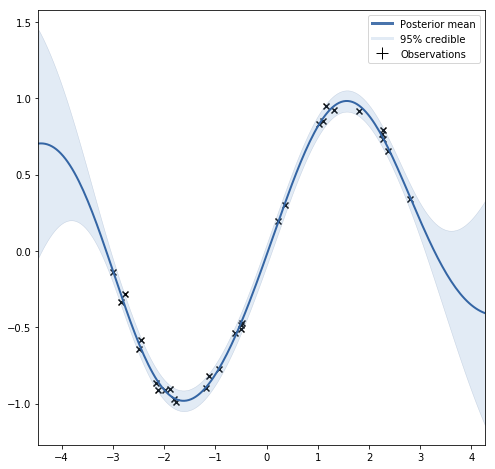
\includegraphics[scale=0.48,width=\textwidth]{figures/high-confidence}
    \caption{Illustration of the 95\% credible intervals for the
    posterior predictive distribution for a regression model. The 
    predictive distribution is narrow, giving tighter
    confidence bands.}\label{fig:high-confidence}
  \end{minipage}
  \hspace{5pt}
  \begin{minipage}{.46\textwidth}
    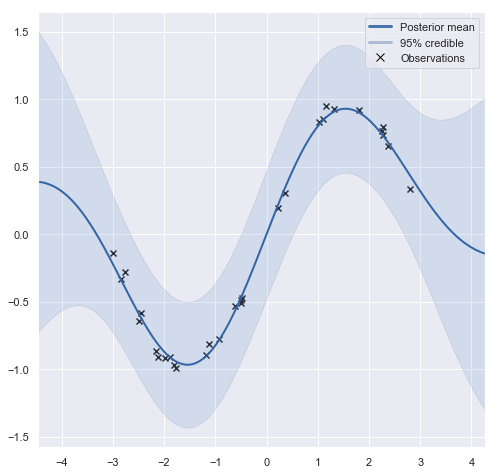
\includegraphics[scale=0.5,width=\textwidth]{figures/low-confidence}
    \caption{Illustration of the 95\% credible intervals for the
    posterior predictive distribution for a regression model. In this
    case the predictive distribution is very wide, giving wider
    confidence bands.}\label{fig:low-confidence}
  \end{minipage}
\end{figure}

which accounts for the parameter uncertainty through the
marginalisation of $\hyperparam$. From the predictive distribution,
very sophisticated predictions can be made. The ``best guess'' of $y$
is represented by $\text{E}[y \vert X]$, and thanks to having
an entire distribution it is possible to compute exactly how certain
it is. This can be done by computing the \textit{credible
  intervals}~\cite{Morey2016Feb} for the distribution, which is the
span in which a certain amount of probability mass lies. For instance,
the 95\%-credible interval would contain 95\% of the probability mass,
which can be interpreted as a 95\% chance of future observations
falling inside this span. An illustration of credible intervals can be seen in
Figure~\ref{fig:high-confidence} and Figure~\ref{fig:low-confidence}.

\section{Arrival Time Prediction}
Arrival time prediction is, in a nutshell, the problem of answering
the question ``When does the bus arrive?''. When viewed as a machine
learning problem, the goal is to
learn a function $\arrtime = f(\obs)$ for arrival time $\arrtime$ and 
state vector $\obs$, which
contains information on the current state of the world. For instance, it
could contain the position of a bus and the time of day.

\subsection{Prediction Evaluation}
The \textit{Mean Absolute Error} (MAE), defined as
\begin{equation}
  \label{eq:mae}
  MAE(\hat{t}, t) = \frac{1}{n}\sum_{i=1}^{n}{\vert \hat{t} - t \vert},
\end{equation}
for true value $\hat{t}$, provides a natural interpretation as 
``the average of the total error'' which is a relevant
and easy-to-understand quantity~\cite{willmott2005advantages}.

%% Two complementary ways of evaluating how good a prediction is are the metrics
%%  (MAE) and \textit{Mean Absolute Percentage
%%   Error} (MAPE), defined for the true value $\hat{t}$ as
%% and
%% \begin{equation}
%%   \label{eq:mape}
%%   MAPE(\hat{t}, t) = \frac{1}{n}\sum_{i=1}^{n} \vert \frac{\hat{t} - t}{\hat{t}} \vert
%% \end{equation}
%% respectively. 

%%  MAPE on the other hand calculates a relative
%% error~\cite{Armstrong1992Jun}, which is unaffected by the
%% magnitude. One issue with it is that it is only defined for $\hat{t}
%% \ne 0$. 
%% These metrics are complementary

\section{Gaussian Processes}
A GP generalises a multivariate normal distribution, and can be seen
as a distribution over functions, completely defined by its
mean function $m(x)$ and covariance function $k(x, x', \hyperparam)$~\cite{Rasmussen-Williams-2006}. 
Here, $x$ and $x'$ are
elements in the domain of modeled functions, and $\hyperparam$ a
vector of hyper-parameters for the covariance function. For any input
vector $x$, the output $y$ is assumed jointly normally distributed according to
\begin{equation}
  \label{eq:gp}
  y = f(x) \sim \mathcal{N}(\mu(x), \Sigma(x))
\end{equation}
where
\begin{equation}
  \label{eq:gp-mean-function}
  \mu(x) = m(x) + K(x, \textbf{x})\textbf{V}^{-1}{(y-m(x))}^{T},
\end{equation}
\begin{equation}
  \label{eq:gp-covariance-function}
  \Sigma(x) = K(x, x) + \sigma^{2}_n\textbf{I} - \textbf{K}(x, \textbf{x})\textbf{V}^{-1}{\textbf{K}(x, \textbf{x})}^{T},
\end{equation}
and $\textbf{K}$ is the gram matrix with elements $K_{ij} = k(x_i, x_j)$ and $\textbf{V}
= K(x, x) + \sigma_n^2I$.
In the context of this thesis, the mean function $m(x)$ can be assumed to be $m(x) = 0$
without loss of generality, making the covariance function $k(x, x', \hyperparam)$
the only free parameter. Picking a specific function represents a prior
belief on how values close in $y$ are related, expressed in $x$. This
concept is explored in more detail in Section~\ref{sec:kernels-as-priors}.
Training a GP is typically done using maximum likelihood
estimation. That is, the GP parameters $\hyperparam$ are optimised to
maximise the data likelihood. Unfortunately, this is non-convex
optimisation problem, so
iterative methods have to be used. The likelihood function is
non-convex, which introduces a high risk of finding local minimas
during the optimisation process. Because of this, random restarts are
typically required to find a good $\hyperparam$.

\subsection{Kernels as Covariance Functions}\label{sec:kernels-as-priors}
Covariance function formalises a prior belief on the shape of the target
function, by specifying how correlated function values $y$ are by
evaluation the kernel function pair-wise on the observarions. 
While in practice any binary function can be plugged into
a GP, a class of functions known as \textit{kernels} are typically
used, since they have useful properties for expressing covariance. In
particular, kernels are positive-definite functions, which in turn
gives a positive-definite covariance matrix. This is required for it
to be invertable, which in turn is required to compute the GP posterior. 
The requirement of positive-definiteness makes intuitive sense, since covariance can not
be negative. 

Kernels are increadibly flexible, and can be defined for other entities than continuous
funtions, such as graphs, strings and
images~\cite{duvenaud2013structure}. However, for this thesis project
only kernels on continuous functions are considered. Kernels on
continuous functions are able to express a wide range of prior beliefs, from linearity to symmetry and
periodicity. Figure~\ref{fig:kernel-priors} illustrates several kernels
found in the literature on continuous functions together with samples from their priors.
\begin{figure}
  \centering
  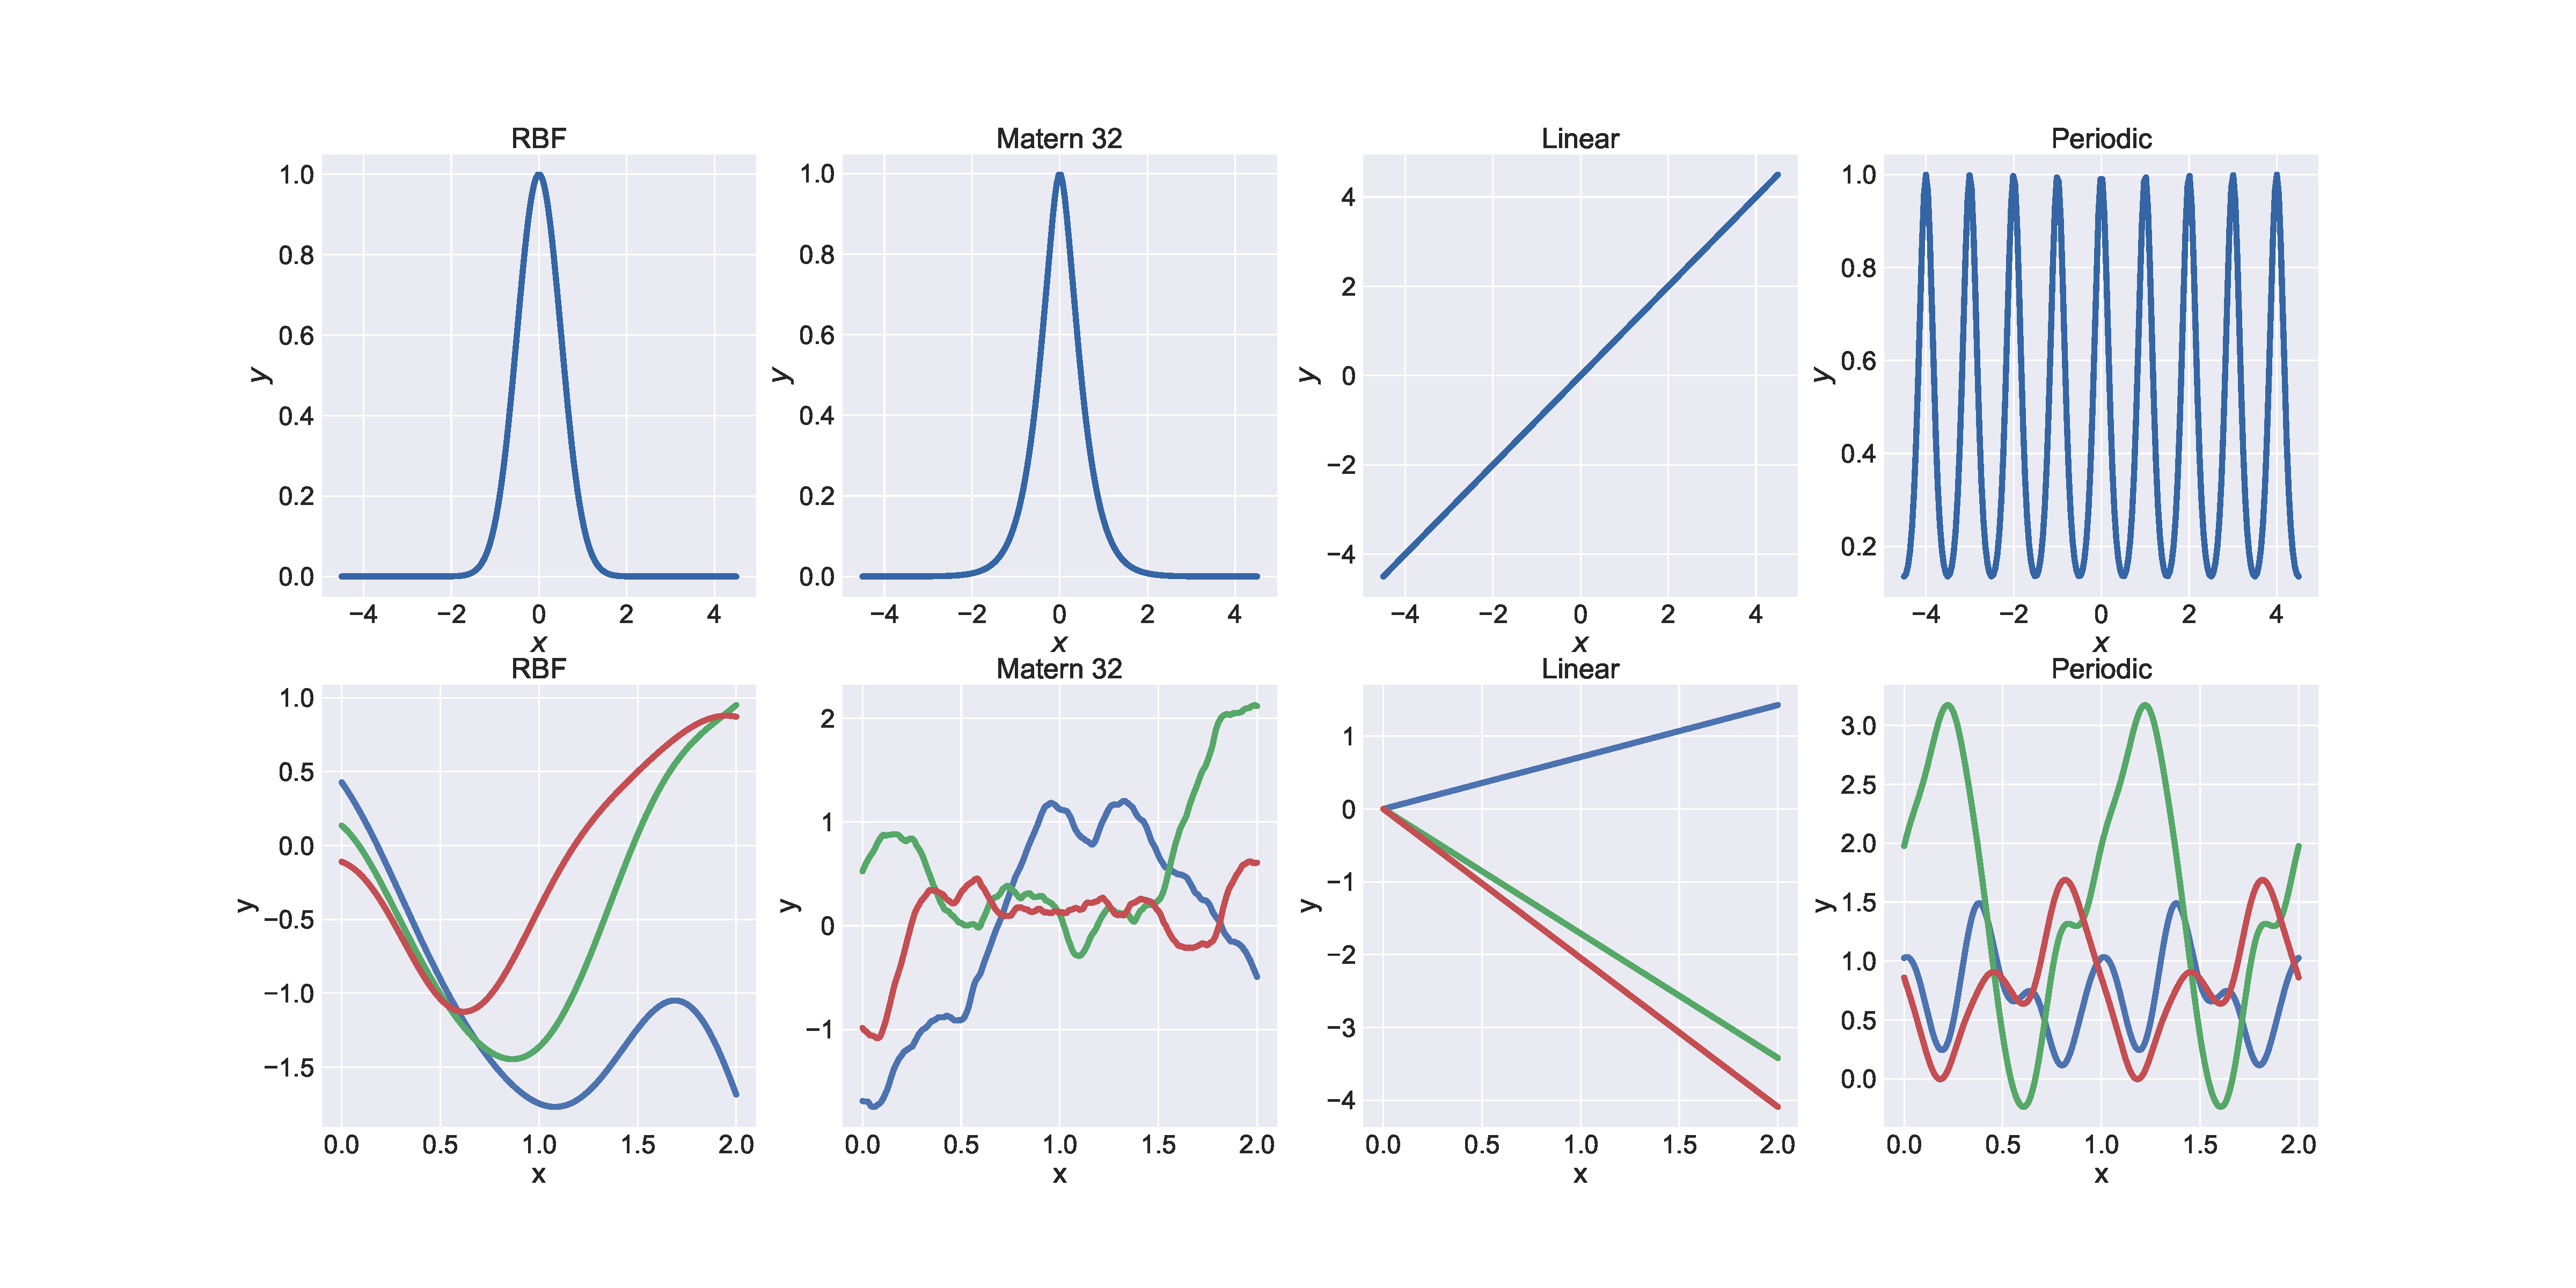
\includegraphics[width=\textwidth]{figures/kernel-priors-vert}
  \caption{Illustration of different kernels and samples from their
    priors. From left to right the kernel functions are RBF (Radial
    Basis Fuction), Matern 32, linear kernel, and periodic kernel.}\label{fig:kernel-priors}
\end{figure}

Even though a single kernel captures a lot of priors, it is sometimes
desireable to express more complicated one. Fortunately,
the set of kernel functions are closed under multiplication and addition, which
creates a principled way of combining them, creating \textit{compound
  kernels}~\cite{duvenaud2013structure}. Kernels can be combined as
required to capture prior beliefs about periodicity \textit{and}
linearity, for instance. Figure~\ref{fig:compound-kernels} illustrates
the concept of compound kernels.
\begin{figure}
  \centering
  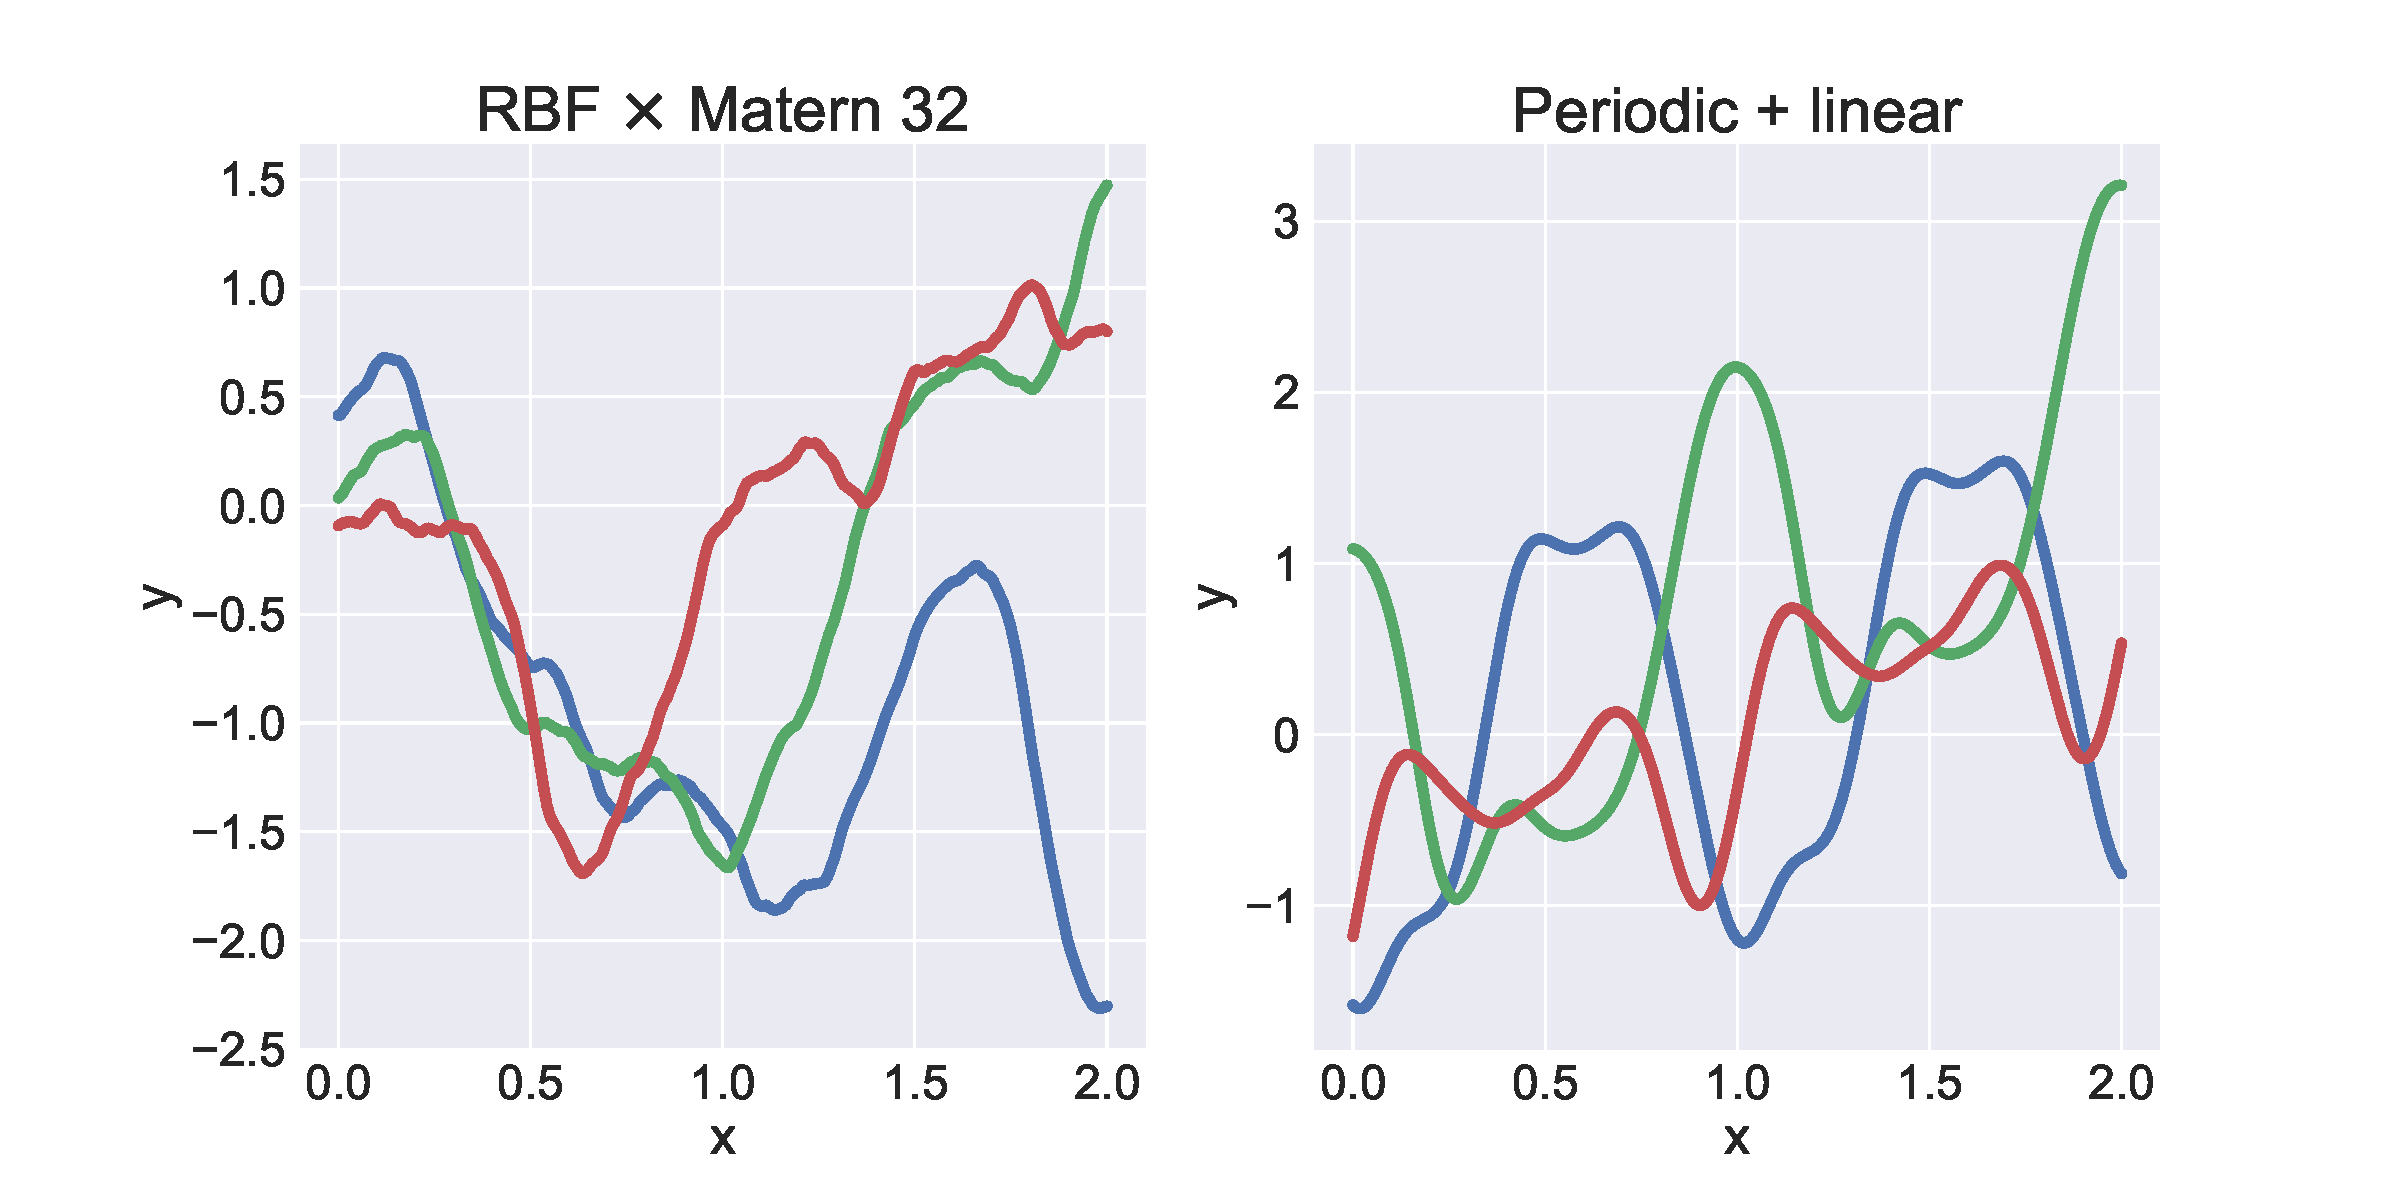
\includegraphics[width=0.75\textwidth]{figures/compound-kernels}
  \caption{Illustration of compound kernels. In the top row RBF
    and Matern 32 are combined by multiplication, and in the bottom
    row a linear and periodic kernel are combined by addition.}\label{fig:compound-kernels}
\end{figure}

\subsection{Structure Discovery Using Gaussian Processes}
Structure discovery is the problem of automatically learning the
structure of data. By creating kernels for specific characteristics
and combining them in a way that maximises the marginal likelihood, it
is possible to detect said characteristics, based on the combination
of kernels~\cite{duvenaud2013structure}.

There are infintely many ways to construct compound kernels, and some
kernel combinations explain a specific data set $X$ better than
other. How well a kernel $k$ explains $X$ can be approximated
by the Bayesian information criterion (BIC)
\begin{equation}
  BIC(k) = \log p(X \vert k) - \frac{1}{2} \vert k \vert \log N,
\end{equation}
where $\vert k \vert$ denotes the number of kernel parameters and $N$
the number of observations. BIC assumes independence between
observations conditioned on parameters, but this is in general not the
case in a GP model. However, it has been shown to be a good enough approximation~\cite{duvenaud2013structure}.
\begin{figure}
  \centering
  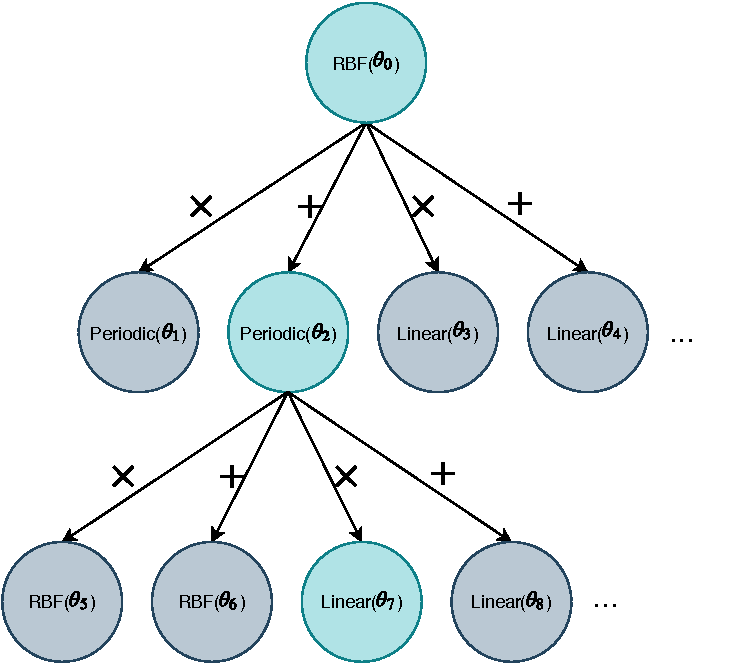
\includegraphics[width=0.75\textwidth]{figures/compound-kernel-search}
  \caption{Illustration of greedy search over kernel structures under
    multiplication and addition, where the
    expanded nodes are highlighted. Each kernels hyperparameters
    $\hyperparam_i$ are learned from data, and the kernel that
    minimises BIC the most is selected.}\label{fig:compound-kernel-search}
\end{figure}

With a way of comparing kernels established, it is interesting to find
\textit{the best} compound kernel for $X$. That is, the kernel
composition that maximises BIC. One way to do so is to
greedily search over a set of pre-defined kernel compositions, fitting
them to data as the search goes, and composing the ones that minimise
the BIS into the compound kernel. This process is illustrated in Figure~\ref{fig:compound-kernel-search}.
The structure of the resulting kernels reveals structure in the
data. For instance, if the resulting kernel contains a RBF component and a periodic
component, the data is locally correlated, and follow a periodic
trend. This process can be used to automatically detect structure in
data, from a cleaverly crafted set of kernels that correspond to
known characteristics.

\section{The Equirectangular Map Projection}
Working with data in latitude-longitude space is tricky, since the two
dimensinos are not scaled 1:1. To make it easier to work with such
data, it can be projected onto a Euclidian space, where it can be
described using cartesian coordiantes. However, since latitude and
longitude describe points on an ellipsis, and cartesian coordiantes are
orthogonal, a perfect projection does not
exist~\cite{snyder1989album}. Because of this, several different
projections have been invented, each making a different trade-off.
One of these is the \textit{Equirectangular Projection}, which maps
latitude $\phi$ and longitude $\lambda$ onto cartesian coordinates $x$
and $y$ through
\begin{equation}
  \label{eq:equirectangular-projection}
  \begin{split}
    x = (\lambda - \lambda_0)&
    \cos \phi_0 \\
    y = (\phi - \phi_0),
  \end{split}
\end{equation}
where $\lambda_0$ and $\phi_0$ define the
central meridian and the standard parallels of the latitude-longitude
space respectively. The projection is
correct for $\phi = \phi_0$, but the further away points are from
$\phi_0$ the larger the residuals will be. The $y$- and $x$--axis of
the resulting cartesian coordinate system will be $\lambda_0$ and
$\phi_0$ respectively.

\chapter{Related Work}
\label{cha:theory}

This section covers related work done on arrival time prediction 
and motion pattern modeling using spatio-temporal data. It
also covers related work relevant to clustering of trajectory data
and to detection of characteristics in motion patterns.

\section{Arrival Time Prediction}
Arrival time prediction is, in a nutshell, the problem of answering
the question ``When does my bus arrive?''. In recent years, machine learning
techniques have been very successful at this task, and Long Short-Term 
Memory Networks (LSTMs) in particular have proven
extremely effective. J.pang et al. predicted bus arrival times to the next station in a
continuous setting using LSTMs given the current position of a bus and static domain knowledge
about its last stop~\cite{pang2018learning}. 
D. Nguyen et al. also used LSTMs, but with entire
trajectories~\cite{Nguyen2018Jun}. They predicted arrival times of
ships by training a model to generate continuations of trajectories, and  
when the model was presented with a new unfinished trajectory, it generated a
probable continuation until it arrived at a port. This was then used to
make its predictions.

While these approaches do perform admirably on test
data, they lack explainability and a way to measure the models certainty.

\section{Motion Pattern Learning}
Motion pattern learning is the problem of learning motion patterns from a
set of trajectories, such that each pattern captures a different
characteristic of the trajectories. An example with synthetic data can be
seen in Figure~\ref{fig:motion-pattern-example}. Note that the term
\textit{Trajectory learning} is often used in the literature for the
same problem, however, the term ``trajectory'' is ambiguous so in the
scope of this thesis the name motion pattern learning will be used. 
\begin{figure}[H]
  \centering
  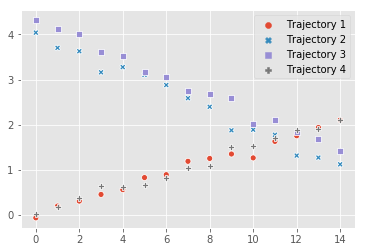
\includegraphics[width=0.7\textwidth]{figures/motion-pattern-example}
  \caption{Synthetic data showing two motion patterns with two trajectories in
    each. Trajectory 2 and 3 belong to one motion pattern and
    Trajectory 1 and 4 belong to a second motion pattern.}\label{fig:motion-pattern-example}
\end{figure}
Motion pattern learning has a natural interpretation as a
clustering problem, but clustering trajectories is difficult,
since different trajectories can have different lengths.
This means that they do not exist in the same vector space and are not
naturally comparable using similarity metrics based on Euclidan
distance. Because of this, more
advanced similarity metrics need to be used. Several different
approaches have been explored, mainly divided by being either deterministic
or probabilistic. Common deterministic techniques
include using spectral clustering with Dynamic Time Warping
(DTW)~\cite{Tang2018Aug} or Longest
Common Subsequence (LCSS)~\cite{Vlachos2002Feb} as similarity metrics.
These similarity metrics are however computationally expensive, making them unsuitable for
real time processing~\cite{Zhang2006Aug}.

\subsection{Probabilistic Approaches}
The probabilistic approach instead fits a model to each motion pattern
and infers its parameters from data. Two popular approaches for this
is fitting Gaussian processes (GPs) and hierarchical Bayesian modeling

\subsubsection{Gaussian Processes}
GPs have been used in several domains for modeling trajectories.
M. Pimentel et al. used GPs to model the vital signs of patients~\cite{Pimentel2013Sep}, 
and were successfully able to cluster the data using hierarchical clustering
and the GP model likelihoods. They then modeled the motion pattern
for a cluster as a GP with the average mean and variance for all GPs in it.
K. Kim. et al. used GPs to model the motion patterns of cars from
surveillance camera~\cite{Kim2011Nov}. They introduce the 
concept of a \textit{frame}, in which the trajectories are
discretisised before fitting GPs to them. Having discrete trajectories meant that
the local likelihood for observed data $x_t, y_t$ in time step $t$
could be computed as $P(y_t | x_t, {M_k})$ for model $M_k$, which
were aggregated to compute a global similarity metric $L_k$,
which in turn was used to cluster the trajectories. To compute the motion
patterns of clusters, a sampling scheme was used. In each time
point, three GPs were drawn uniformly without replacement from the
cluster. The mean value of all drawn GPs were then used as data points
to fit a GP for the clusters motion pattern.

Q. Tran and J. Firl used data with both spatial position and velocity,
and used GPs to model a vector field for each observed
trajectory~\cite{Tran2014Jun}. Before GPs were trained, the trajectories 
were normalised using spline interpolation and a
sampling scheme. They did not perform any clustering. Instead, they
constructed their motion patterns by driving their own test vehicle. 
When presented with a new trajectory, the model could then compute the most
likely motion pattern, and then use a particle filter for the vector
field to predict continuations of motion patterns.

The work of M. Tiger and F. Heintz aimed to improve upon the approach of K. Kim et
al. who had implicitly assumed that all trajectories were generated
from one underlying processes, while a more accurate model is
that they are generated from several different, but dependent
processes. Assuming a single underlying process causes the model to
underestimate its variance, which in turn causes the models likelihood
to be too small for data that is still fairly close.
They aggregated clustered GPs by considering the mixture of
Gaussian distributions they form in a ``slice'', orthogonal to
progression. These slices were then combined to form a single Gaussian
distribution. They then generated synthetic data and learned
hyperparameters for a single GP to approximate the combined Gaussian
distribution, a process they call ``inverse Gaussian process regression''.

C. Leysen et al. also aim to improve on the work of K. Kim et
al~\cite{Leysen2016Sep}. Instead of fitting a GP to re-sampled trajectories, 
they simply select the trajectory in a cluster which maximises the overall
likelihood of the data points in the cluster. While this is less
ad hoc, their approach still assumes a single underlying function for
all trajectory data, and consequently still underestimates model variance.

\subsubsection{Hierarchical Bayesian Models}
The idea behind Hierarchical Bayesian Models used for trajectory
learning is borrowed from the natural language processing field, where
they are known as topic modeling. Topic modeling are unsupervised
techniques for clustering documents into different topics, and by 
considering spatio-temporal trajectories as documents,
their observations as words, and the motion patterns they belong to as
topics, the same techniques can be used to model motion pattern.  
These models are usually based on Latent Dirichlet Allocation (LDA) or
a generalisation thereof known as Hierarchical Dirichlet Process (HDP)
introduced by Teh et al.~\cite{teh2005sharing}, which are both so called \textit{bag-
of-words}-models. A bag-of-words-model assumes independence between
words in a document, which in the domain of trajectories translates to the
assumption that observed data points are independently drawn.

Both LDA and HDP require a set amount of clusters, which is a great
weakness. Wang et al. proposed a model called \textit{Dual Hierarchical Dirichlet
Process} (Dual-HDP)~\cite{Wang2008Jun}, which improves upon the HDP model
by allowing the model to learn the number of topics and documents from
data. Zhou et al. improved upon HDP and LDA by using Markov random
fields to encode prior beliefs in a model called \textit{Random Field
  Topic} (RFT)~\cite{Zhou2011Jun}.

-- this is more recent but I have not been able to figure this paper out yet--
LC-LDA~\cite{Zou2016Apr}

%~\cite{Campo2017Aug}

% HMM on human writing~\cite{Suzuki2007Oct}

% Gaussian Process regression has been used to model trajectories in
% different domains. Medical domain 

% Gaussian Process regression flow in a frame. Requires synchronised
% trajectories and  There  are  some  limitations  and  avenues  of  improve-
% ments.  First, our approach assumes that the types of nor-mal patterns are defined
% a priori. Secondly, if the trajectory is too sparse, 
% the kurtosis measurements in earlier stages of
% the track can be unstable due to the sensitivity of kurtosis
% in a sparse distribution. Finally, our approach does not rec-
% ognize traffic jams and such patterns would be detected as
% an anomaly. A traffic jam, however, can be represented as a
% step shape function in the normalized(u,v,t)coordinates,
% and we plan to use this method to model traffic jams.~\cite{Kim2011Nov}

% similarities (time, space), differences (no frames)

% \subsection{Trajectory Clustering}

% \subsection{Motion Pattern Modeling}


% \section{Motion Pattern Characteristics Detection}


% The main purpose of this chapter is to make it obvious for
% the reader that the report authors have made an effort to read
% up on related research and other information of relevance for
% the research questions. It is a question of trust. Can I as a
% reader rely on what the authors are saying? If it is obvious
% that the authors know the topic area well and clearly present
% their lessons learned, it raises the perceived quality of the
% entire report.

% After having read the theory chapter it shall be obvious for
% the reader that the research questions are both well
% formulated and relevant.

% The chapter must contain theory of use for the intended
% study, both in terms of technique and method. If a final thesis
% project is about the development of a new search engine for
% a certain application domain, the theory must bring up related
% work on search algorithms and related techniques, but also
% methods for evaluating search engines, including
% performance measures such as precision, accuracy and
% recall.

% The chapter shall be structured thematically, not per author.
% A good approach to making a review of scientific literature
% is to use \emph{Google Scholar} (which also has the useful function
% \emph{Cite}). By iterating between searching for articles and reading
% abstracts to find new terms to guide further searches, it is
% fairly straight forward to locate good and relevant
% information, such as

% Having found a relevant article one can use the function for
% viewing other articles that have cited this particular article,
% and also go through the article’s own reference list. Among
% these articles on can often find other interesting articles and
% thus proceed further.

% It can also be a good idea to consider which sources seem
% most relevant for the problem area at hand. Are there any
% special conference or journal that often occurs one can search
% in more detail in lists of published articles from these venues
% in particular. One can also search for the web sites of
% important authors and investigate what they have published
% in general.

% This chapter is called either \emph{Theory, Related Work}, or
% \emph{Related Research}. Check with your supervisor.



\chapter{Data}
Explain one observation per second
Explain the clusters at stops
\chapter{Method}
\label{cha:method}
This chapter describes the proposed system for arrival time prediction
and event detection, and its implementation.

\section{System Description}
This section formally describes the system piece-wise. On a conceptual
level, the system assumes that similar trajectories, with respect to their motion patterns, should arrive at
approximately the same time. When presented with a new trajectory, the system
finds previously observed trajectories with similar motion patterns,
and predict arrival times based on the most similar one. 

The current system description assume that each trajectory represents
a motion pattern (motion pattern clusters has a single trajectory).

\section{Trajectory Model}
To find similar trajectories, a trajectory similarity metric 
is needed. The similarity metric need to be well defined for
trajectories of different temporal lengths, and unevenly
distributed observations.

\subsection{Synchronisation Model}
One notion of similarity between trajectories is some aggregation of
local similarities. Consider the local distance from an observation on trajectory
$\traj_2$ to trajectory $\traj_1$ as the distance of the orthogonal
projection onto $\traj_1$, as illustrated in Figure~\ref{fig:trajectory-projection}.
\begin{figure}
  \centering
  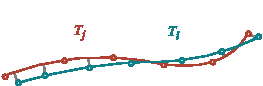
\includegraphics[scale=2.5]{trajectory-projection}
  \caption{An illustration of local distances from $\traj_2$ to
  $\traj_1$ as point-wise orthogonal projections.}\label{fig:trajectory-projection}
\end{figure}
This approach would eliminate the need to align observations before
comparison. However, it requires a continuous trajectory
representation, while trajectories are observed as discrete samples.
A step toward this is seeing observations as samples from a continuous function
$\traj_{k} = \tilde{f}_{k}(t)$, which describes the trajectory as a function of
time. While continuous, this description is based on specific time
points, but the \textit{exact points in time} of observations are not
relevant, since trajectories for a single segment are generated at many different
occasions. Instead, consider observations as samples from the function
as $\traj_{k} = \modelf_{k}(\synchspace)$, where $\synchspace = [0, 1]$ is the \textit{progress} from
start ($\synchspace = 0.0$) to finish ($\synchspace = 1.0$) of
a trajectory. This function makes it possible to talk about observations based on
progression for any trajectory, regardless of the exact observation time points. 

Assuming the samples are jointly Normally distributed, and
that $\modelf$ is smooth, a GP can be fit to the
observations to approximate $\traj_{k} = \modelf_{k}(\synchspace)$, with
independent outputs. Finding a projection for an observation $\newobs$ onto trajectory
$\traj_{k}$ can now be seen as finding how far along the trajectory $\newobs$
would have traveled. More precisely, finding the $\tau$ that $\newobs$
corresponds to. Under the assumption that $\synchspace \sim
\mathcal{N}(\mu_{\synchspace}, \Sigma_{\synchspace})$, a multivariate
GP is used to model $\synchspace = \synchf_{k}(\obs)$, which maps $\newobs$ onto the
progress relative to $\traj_{k}$. When considering progress along a
segment, the current velocity does not matter. Hence, the domain of
$\synchf_{k}$ is the subspace $S' = (p_x, p_y)$ of $S$, and
consequently $S$ is collapsed into $S'$ before mapping onto $\synchspace$. The projection onto $\traj_{k}$ is
finally given by the composition $\synchedobs = (\modelf \circ
\synchf)(\obs)$, illustrated in Figure~\ref{fig:synch-model}.
\begin{figure}
  \centering
  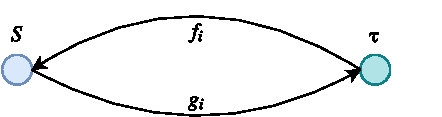
\includegraphics[scale=1.5]{synch-model}
  \caption{An illustration of the mappings involved when synchronising
    trajectories. Observations are first projected by $p$ from $S$ onto the
    subspace $S'$, spanning only the dimensions $p_x, p_y$. Then onto
    $\synchspace$ by $\synchf_{k}$, and finally back onto $S$ by
    $\modelf_{k}$.}\label{fig:synch-model}
\end{figure}
In light of the these results, let $\model_{synch}^{(k)} = (\modelf_{k},
\synchf_{k})$ be the \textit{synchronisation model} of $\traj_{k}$.
The final step is to formulate a local similarity metric from the
projections and aggregate this into a global one.
While it is intuitive to define the local similarity as the absolute difference $|E[\synchedobs]
- \newobs$|, this approach does not consider the  uncertainty in $\synchedobs$. 
Consider instead the data log likelihood
\begin{equation}
  \label{eq:model-log-likelihood}
  \begin{split}
    \log P(\synchspace|\newobs, \model_{synch}^{(k)})
    & = -\frac{1}{2}(\synchspace - \mu(\newobs)){[\Sigma(\newobs)]}^{-1}(\synchspace - \mu(\newobs)) \\
    & = -\frac{1}{2}\log{|\Sigma(\newobs)|}+C,
  \end{split}
\end{equation}
where $\mu(\newobs)$ and $\Sigma(\newobs)$ are given by
equations~\ref{eq:gp-mean-function},
and~\ref{eq:gp-covariance-function} for a GP modeling $f_{k}$. The
likelihood measures how well $\model_{synch}^{(k)}$ explains observation
$\newobs$, and is a measure of similarity. Assuming that all models
are equally probable a priory, Bayes theorem gives
\begin{equation}
  \label{eq:model-posterior}
  \begin{split}
    \log P(\model_{synch}^{(k)} | \newobs, \synchspace)
    & \propto \log P(\synchspace|\newobs, \model_{synch}^{(k)}) + \log
    P(\model_{synch}^{(k)}) \\
    & \propto \log P(\synchspace|\newobs, \model_{synch}^{(k)})
  \end{split}
\end{equation}
and the most similar model can consequently be chosen by $M_{c} = \underset{k}{\mathrm{argmax}} \log
P(\model_{synch}^{(k)} | \newobs, \synchspace)$. Having a distribution
over models will also prove useful when making arrival time
predictions. This local similarity measure generalises to a global one
for an entire trajectory by letting $\newobs$ be
\[\newobs =
  \begin{pmatrix}
    p_{x}^{1} & p_{y}^{1} & v_{x}^{1} & v_{y}^{1} \\
    p_{x}^{2} & p_{y}^{2} & v_{x}^{2} & v_{y}^{2} \\
    \vdots  & \vdots  & \vdots & \vdots  \\
    p_{x}^{m} & p_{y}^{m} & v_{x}^{m} & v_{y}^{m} \\
  \end{pmatrix}.
\]

\subsection{Learning the Synchronisation Model}
Learning a synchronisation model $\model_{synch}^{(k)}$ means learning
$\modelf_{k}$ and $\synchf_{k}$ by MAP estimation. However, there are
more constraints on the functions than can be formulated in
priors. In particular, a critical property of $\synchf_{k}$
is that it should be monotonically increasing in the direction of progression,
and stationary orthogonal to it. This is intuitively explained by the fact that a
vehicle is no closer to its destination should it drive more to the
left or right on a road; only the progression \textit{along} the road
matters. Formally, this is required for the projection onto a
trajectory to be orthogonal. To enforce this property, data augmentation is used.

When training GPs using a stationary kernel function, it is assumed
that the data is uniformly distributed, which is not the case for the
data set used. Recall the function $\synchf_{k} : \posspace \mapsto
\synchspace$. In this case, the data is assumed to be uniformly
distributed in $\posspace$, but as described in Chapter~\ref{ch:data},
all data is collected approximately uniform in \textit{time}. This causes many
observations to be generated in close proximity during stand-stills, which skews the
learning of the kernel lengthscale parameters to small values. To
make data approximately uniformly distributed spatially instead and 
avoid this problem, a technique called \textit{stop compression} is used.

\subsubsection{Data Augmentation}
\label{sec:data-augmentation}
For reasons previously described, $\synchf_{i}$ should be monotonically increasing in
the direction of progression and stationary orthogonal to it.
To enforce learning such a function, each
observation $\obs_{i}^{(i)}$ for a trajectory $\traj_{i}$is duplicated by placing a normal distribution
over it, orthogonal to the spatial progression vector ${(\obs^{(i+1)}_x -
  \obs^{(i)}_x, \obs^{(i+1)}_y - \obs^{(i)}_y)}^T$, and drawing several samples
with the same progression as $\obs^{(i)}$. This process is illustrated in
Figure~\ref{fig:traj-without-support-data} and
Figure~\ref{fig:traj-with-support-data}.
\begin{figure}
  \begin{minipage}{.46\textwidth}
    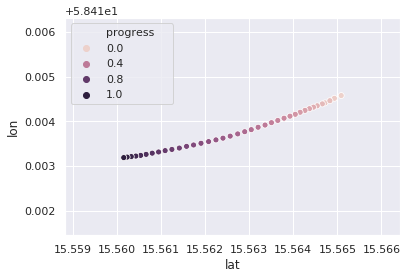
\includegraphics[scale=0.48,width=\textwidth]{traj-without-support-data2}
    \caption{Spatial progression of a trajectory
      before data augmentation.}\label{fig:traj-without-support-data}
  \end{minipage}
  \hspace{5pt}
  \begin{minipage}{.46\textwidth}
    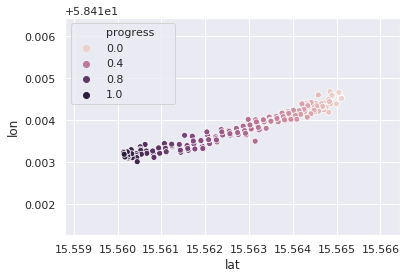
\includegraphics[scale=0.5,width=\textwidth]{traj-with-support-data2}
    \caption{Spatial progression of a trajectory
      after data augmentation. }\label{fig:traj-with-support-data}
  \end{minipage}
\end{figure}

\subsubsection{Stop Compression}
\label{sec:stop-compression}
Stop compression aggregates observations in close proximity into a
single observation through averaging. Observations within a radius of
$4$m are clustered into a single observation with the mean value of
the clustered observations. An example of this is seen
Figure~\ref{fig:stop-compression-before} and Figure~\ref{fig:stop-compression-after}.
\begin{figure}
  \begin{minipage}{.46\textwidth}
    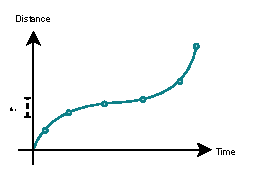
\includegraphics[scale=0.48,width=\textwidth]{stop-compression-before}
    \caption{Trajectory before stop compression. Several observations
      are very close spatially, but the data is
      approximately uniformly distributed temporally. }\label{fig:stop-compression-before}
  \end{minipage}
  \hspace{5pt}
  \begin{minipage}{.46\textwidth}
    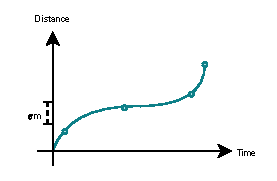
\includegraphics[scale=0.5,width=\textwidth]{stop-compression-after}
    \caption{Spatial progression of a trajectory
      after stop compression. The data is
      approximately uniformly distributed spatially.}\label{fig:stop-compression-after}
  \end{minipage}
\end{figure}

\subsection{Prediction Model}
Predicting arrival times can be seen as learning the remaining time of
a segment given a certain position. However, modeling it as $\arrtime
= \tilde{\predf_{k}}(p_x, p_y)$ would assume that every trajectory passes the
exact same positions. A better model is $\arrtime
= \predf_{k}(\synchspace)$, which instead depends on progression. Since the
progression represents similar trajectories and not a single one, this
model generalises much better. Assuming that $\arrtime \sim
\mathcal{N}(\mu_{\arrtime}, \Sigma_{\arrtime})$, a GP can model $\predf_{k}$, 
extending the synchronisation model to the \textit{trajectory model}
$\model_{k} = (\modelf_{k}, \synchf_{k}, \predf_{k})$, illustrated in Figure~\ref{fig:trajectory-model}.
\begin{figure}
  \centering
  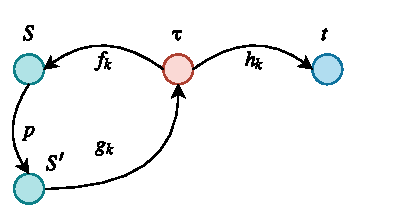
\includegraphics[scale=1.5]{trajectory-model}
  \caption{An illustration of the trajectory model, which models
    current state $S$ and time left $\arrtime$ as functions of
    progress $\synchspace$. $P$ denotes orthogonal projection.}\label{fig:trajectory-model}
\end{figure}

\section{Arrival Time Predictions}
The arrival time predictions are modeled as a Mixture of Gaussian
Processes (MoGP), where each motion pattern model $\model_{k}$ induce a component. The
model predicts remaining time until arrival, and the probability of
the time remaining being $t$ for an observation $\obs$ is given by
the mixture
\begin{equation}
  P(\arrtime | \obs) = \sum_{k}P(\arrtime | \obs, \model_{k}) P(\model_{k}),
\end{equation}
where the component weights $P(\model_{k})$ are given by
equation~\ref{eq:model-posterior}. Since all components are Gaussian, 
$P(\arrtime | \obs)$ will have one mode for each component. The
point-estimate prediction of the model is taken to be the largest
mode, corresponding to the mean prediction of the most probable model.

% \begin{figure}[H]
%   \begin{minipage}{.46\textwidth}
%     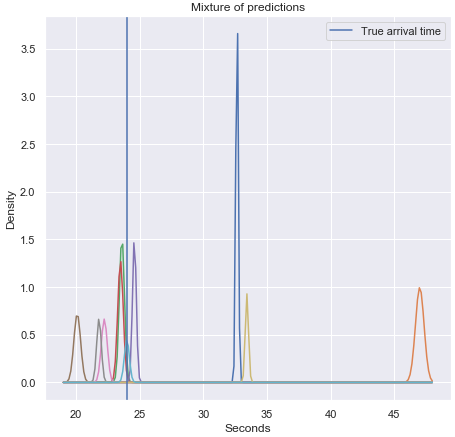
\includegraphics[width=\textwidth]{figures/mixture-start-of-traj.png}
%     \caption{Density of arrival time predictions at 
%       the start of a segment.}\label{fig:mixture-start-of-traj}
%   \end{minipage}
%   \hspace{5pt}
%   \begin{minipage}{.46\textwidth}
%     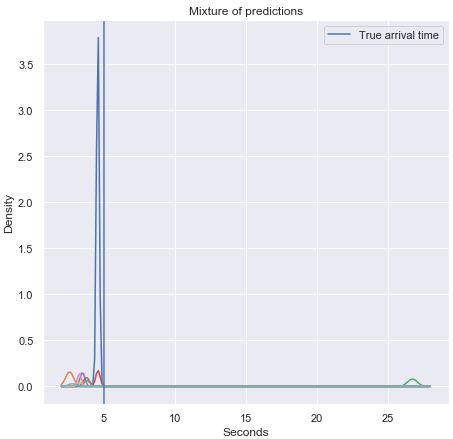
\includegraphics[width=\textwidth]{figures/mixture-end-of-traj.png}
%     \caption{Density of arrival time predictions at 
%       the end of a segment.}\label{fig:mixture-end-of-traj}
%   \end{minipage}
% \end{figure}

\subsection{Event Detection}
The problem of detecting events have not yet been investigated.
\chapter{Results}
\label{cha:results}

% This chapter presents the results. Note that the results are presented
% factually, striving for objectivity as far as possible.  The results
% shall not be analyzed, discussed or evaluated.  This is left for the
% discussion chapter.

% In case the method chapter has been divided into subheadings such as
% pre-study, implementation and evaluation, the result chapter should
% have the same sub-headings. This gives a clear structure and makes the
% chapter easier to write.

% In case results are presented from a process (e.g. an implementation
% process), the main decisions made during the process must be clearly
% presented and justified. Normally, alternative attempts, etc, have
% already been described in the theory chapter, making it possible to
% refer to it as part of the justification.


\chapter{Discussion}
\label{cha:discussion}
klustering av rörelsemönster
mängden data som används, inducing inputs


% This chapter contains the following sub-headings.

% \section{Results}
% \label{sec:discussion-results}

% Are there anything in the results that stand out and need be
% analyzed and commented on? How do the results relate to the
% material covered in the theory chapter? What does the theory
% imply about the meaning of the results? For example, what
% does it mean that a certain system got a certain numeric value
% in a usability evaluation; how good or bad is it? Is there
% something in the results that is unexpected based on the
% literature review, or is everything as one would theoretically
% expect?

% \section{Method}
% \label{sec:discussion-method}

% This is where the applied method is discussed and criticized.
% Taking a self-critical stance to the method used is an
% important part of the scientific approach.

% A study is rarely perfect. There are almost always things one
% could have done differently if the study could be repeated or
% with extra resources. Go through the most important
% limitations with your method and discuss potential
% consequences for the results. Connect back to the method
% theory presented in the theory chapter. Refer explicitly to
% relevant sources.

% The discussion shall also demonstrate an awareness of methodological
% concepts such as replicability, reliability, and validity. The concept
% of replicability has already been discussed in the Method chapter
% (\ref{cha:method}). Reliability is a term for whether one can expect
% to get the same results if a study is repeated with the same method. A
% study with a high degree of reliability has a large probability of
% leading to similar results if repeated. The concept of validity is,
% somewhat simplified, concerned with whether a performed measurement
% actually measures what one thinks is being measured. A study with a
% high degree of validity thus has a high level of credibility. A
% discussion of these concepts must be transferred to the actual context
% of the study.

% The method discussion shall also contain a paragraph of
% source criticism. This is where the authors’ point of view on
% the use and selection of sources is described.

% In certain contexts it may be the case that the most relevant
% information for the study is not to be found in scientific
% literature but rather with individual software developers and
% open source projects. It must then be clearly stated that
% efforts have been made to gain access to this information,
% e.g. by direct communication with developers and/or through
% discussion forums, etc. Efforts must also be made to indicate
% the lack of relevant research literature. The precise manner
% of such investigations must be clearly specified in a method
% section. The paragraph on source criticism must critically
% discuss these approaches.

% Usually however, there are always relevant related research.
% If not about the actual research questions, there is certainly
% important information about the domain under study.

% \section{The work in a wider context}
% \label{sec:work-wider-context}

% There must be a section discussing ethical and societal
% aspects related to the work. This is important for the authors
% to demonstrate a professional maturity and also for achieving
% the education goals. If the work, for some reason, completely
% lacks a connection to ethical or societal aspects this must be
% explicitly stated and justified in the section Delimitations in
% the introduction chapter.

% In the discussion chapter, one must explicitly refer to sources
% relevant to the discussion.

\chapter{Conclusion}
\label{cha:conclusion}

% This chapter contains a summarization of the purpose and the research
% questions. To what extent has the aim been achieved, and what are the
% answers to the research questions?

% The consequences for the target audience (and possibly for researchers
% and practitioners) must also be described. There should be a section
% on future work where ideas for continued work are described. If the
% conclusion chapter contains such a section, the ideas described
% therein must be concrete and well thought through.

\printbibliography
\end{document}